\documentclass[a4paper, 11pt, titlepage, final]{article}[3. prosinec 2011]

\newcommand{\LT}{$<$}
\newcommand{\GT}{$>$}

\usepackage[left=2cm,text={16cm, 25cm},top=2cm]{geometry}
\usepackage[english]{babel}
\usepackage[latin2]{inputenc}
\usepackage[IL2]{fontenc}
\usepackage[dvipdf]{graphicx}
\usepackage{color}

\newcommand{\url}[1]{\textit{#1}}

\title{Documentation for VYPe}
\author{Vendula Poncov�}
\date{\today}

\begin{document}

%%%%%%%%%%%%%%%%%%%%%%%%%%%%%%%%%%%%%%%%%%%%%%%%%%%%%%%%%%%%%%%%%%%%%%%%%
% titulni strana - DON'T TOUCH! MAGIC!

\begin{titlepage}
\begin{center}

{\textsc
{\LARGE Faculty of Information Technology \medskip\\
Brno University of Technology}}

\vspace{\stretch{0.191}}

{\centering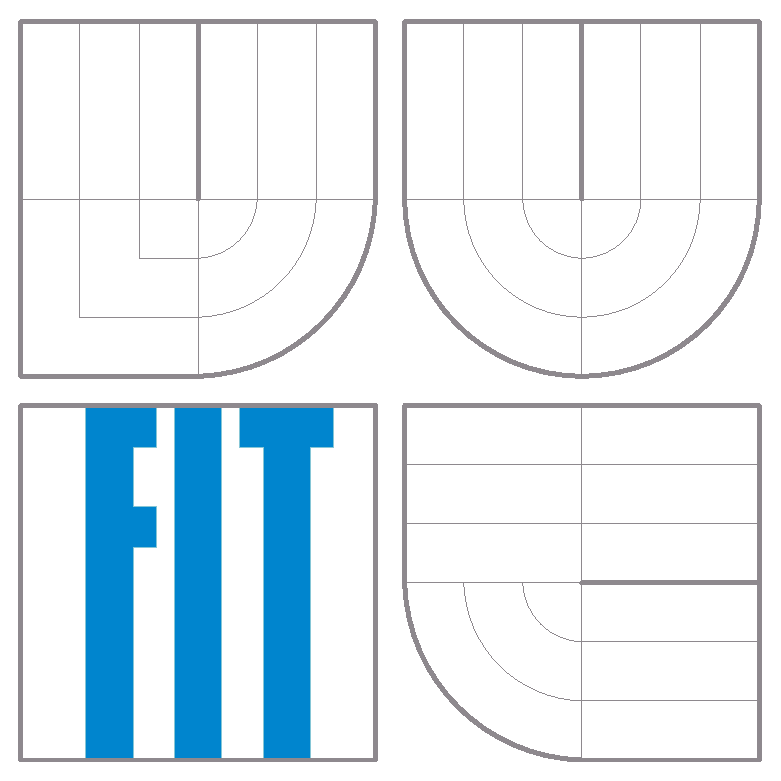
\includegraphics[height=5cm]{img/logo.eps}}

\vspace{\stretch{0.191}}

{{\Huge Documentation for VYPe}} \bigskip

\vspace{\stretch{0.618}}

\end{center}

{\Large
\begin{tabular}{lll}
  Vendula Poncov� & \texttt{xponco00} & 75\% \\
  Martin �ifra & \texttt{xsifra00} & 25\% \\
\end{tabular}
}{\Large \hfill \today}


\end{titlepage}

%%%%%%%%%%%%%%%%%%%%%%%%%%%%%%%%%%%%%%%%%%%%%%%%%%%%%%%%%%%%%%%%%%%%%%%%%
% text dokumentace

\pagestyle{plain}
\pagenumbering{arabic}
\setcounter{page}{1}

%------------------------------------------------------------------------
\section{Introduction}

In this documentation, we describe the design and implementation of the compiler of the programming language \texttt{VYPe2014}.

%------------------------------------------------------------------------
\section{Lexer and parser}

As the front part of our compiler, we have used tools \texttt{flex 2.5.35} and \texttt{bison 2.5}. We were going to implement the compiler in \texttt{C++}, thus we have worked with \texttt{C++} interface in \texttt{bison}. However, \texttt{flex} does not support \texttt{C++} very well, so we have used \texttt{C} interface. The current version of bison is \texttt{3.0.2}, but \texttt{merlin} does not support it.

Lexical analyser is described in file \texttt{lexer.l}, where we define the regular expressions of lexems for \texttt{VYPe2014}. The most challenging were expressions for string and character literals and skipping the comment. For comments, we use state \texttt{COMMENT}, that allows us to ignore characters until we reach the end of the comment. For string and character literals, we explicitly enumerate allowed \texttt{ASCII} codes and escape characters.

Syntax analyser is defined in file \texttt{parser.yy}, where there are definitions of tokens and grammar rules with actions. We have  implemented no extension, thus it was not difficult to design the grammar. The description of the grammar can be found at the page \pageref{grammar}. We skiped the rules for expression.

%------------------------------------------------------------------------
\section{Compiler and generator}

\subsection{Symbol table}

Our symbol table consists of a table of functions and tables of variables. Every function holds a list of tables of local variables. In this way, we can deal with overlapping variable names in nested blocks of statements. We use an auxiliary stack, where we push or pop the pointers to variable tables, when we enter or leave a block of statements. When we need to check if the variable was already defined, we search the tables in the stack from top to down. If there is a variable that overlaps with another variable, we will find the one in the most nested block.

Variables in a variable table hold their name, type and sometimes their value. Functions holds their identifier, list of variables, that are parameters, instructions of three-address code and two flags. One flag symbolizes that the function was declared but not defined, second flag symbolizes, that the function is built-in.

We use the symbol table for semantic analyses. After the semantic error, we always recover and continue with the compilation.

\subsection{Three-address code}

In the syntax analyser, we create three-address code from parse tree. The code is represented by a list of simple instructions. We use several types of instructions. Instruction label represents a place in a code, where we can jump. Instruction expression represents an arithmetical or logical operation between two variables, where the result of the operation is stored in the third variable. For these result variables we generate temporal variables. Cast instruction represents a cast of the variable to another type. There are mentioned three ways of casting in the assignment, however, in the example is also a cast from integer to integer, so we accept a cast to same type as the type of variable as well. Load instruction allows to save a constant value into a variable. Assignment instruction assigns a value from one variable to another. Jump instruction jumps to a label, jump-if-false instruction jumps to label, if the variable is false. Call instruction calls a function with some parameters and stores the result into a temporal variable. Return instruction returns a value of a variable and exits the function.

\subsection{Generating assembly}

Assembly is generated from the tree-address code. We had to implement our own stack, so we can call functions. The target code starts at the function main, pushes all local variables of main on the stack and runs the instructions of the main function. If another function is called, we push the parameters, the value of instruction pointer and the value of context pointer on the stack, set the context pointer on the top of stack and jump to the function. The function pushed all local variables on the stack and set parameters with the values on the stack. When the function returns, it sets the top of the stack to the value of the current context pointer, restores the context pointer and instruction pointer, pushes the result on the stack and jumps back to the caller.

One of the problems of generating target code was storing strings. However, we have noticed, that string cannot be ever modified. Therefore, we can store string variables as pointers to strings and when we assign one string variable to another, we just set the pointer. Variables set to string literal can just point to a constant defined in a memory. String parameters can be passed by reference. The only exception is the return value of the called function. When the function returns string, it has to be copied to the stack, so it will not be lost, when we pop the context.


\subsection{Implementation}

We have implemented the compiler in \texttt{C++}.

Errors are handled in a file \texttt{error.cpp}, where there are defined macros for errors and debugging. The first error code is stored in a static variable and returned as the return value of our program.

Symbol table is implemented in a file \texttt{symtable.cpp}. There are defined classes \texttt{Variable}, \texttt{VariableTable}, \texttt{Function}, \texttt{FunctionTable} and \texttt{SymbolTable} and two enums \texttt{Type} and \texttt{Operation}. The variable and function tables are implemented as maps from the library \texttt{std}.

Classes representing the three-address instructions are defined in a file \texttt{instruction.cpp}. All instructions inherits from class \texttt{Instruction}. Every instruction has implemented a method \texttt{generate}, that returns a string with generated assembly code.

The parsing is driven by a class \texttt{Driver} from file \texttt{driver.cpp}. Driver runs the parsing, generate the three address code and works with a symbol table. The instance of this class is a parameter of the parser and the lexer, thus they can use methods from this class.

If the parsing is finished with success, we call the \texttt{Generator} from file \texttt{generator.cpp}, that accepts the output file and a symbol table of functions and generates assembly. As we mentioned before, most of the generating is defined in a file with instructions.

The program starts in a file \texttt{vype.cpp}. It processes parameters, runs driver and generator and returns a return value.

%------------------------------------------------
\section{Running the program}

The program can be compiled by command \texttt{make}. It creats the file \texttt{vype} as required.

We have written a testing script in \texttt{Python 3.2} and prepared about 80 tests in a folder \texttt{test}. The command \texttt{make test} will run all the tests and show the results. 

%------------------------------------------------------------------------
\section{Division of work}



\begin{tabular}{ll}\\
Vendula Poncov� & lexical analyser \\
                & syntax analyser \\
                & three-address code \\
                & compilation driver \\
                & documentation \\
                & tests \medskip \\
Martin �ifra    & code generator\\
\end{tabular}
\par


%------------------------------------------------------------------------
\section{Summary}

We have implemented the compiler for the programming language \texttt{VYPe2014}. For lexical and syntax analysis, we have used \texttt{flex} and \texttt{bison}. Compiler and generator are implemented in \texttt{C++}.

\newpage
%%%%%%%%%%%%%%%%%%%%%%%%%%%%%%%%%%%%%%%%%%%%%%%%%%%%%%%%%%%%%%%%%%%%%%%%%
% p��lohy

\appendix

%------------------------------------------------------------------------
\section{Grammar} \label{grammar}

{ \tabcolsep=6pt
{\small
 \begin{tabular}{lrrccl}
    &\multicolumn{5}{l}{{G = (N, T, P, S), kde:}} \smallskip \\ 

&\multicolumn{5}{p{17cm}}{{N = \{ \LT program\GT, \LT functions\GT, \LT fce\_declaration\GT, \LT fce\_definition\GT, \LT stmt\_list\GT, \LT stmt\GT, \LT type\GT, \LT datatype\GT,\LT datatype\_list\GT, \LT id\_list\GT, \LT param\_list\GT, \LT argument\_list\GT, \LT expr\_list\GT   \} }} \smallskip \\ 

&\multicolumn{5}{l}{{T = \{ $($, $)$, $\{$, $\}$, $\textit{;}$ , id, $\textit{,}$ , =, if, else, while, return, void, int, char, string \}}} \smallskip \\ 

&\multicolumn{5}{l}{{S = \LT program\GT}} \smallskip \\ 

&P = \{ \\

&&\LT program\GT &$\longrightarrow$& & \LT functions\GT \\

&&\LT functions\GT &$\longrightarrow$& & $\epsilon$ \\
&&  &  & $|$ & \LT fce\_declaration\GT \LT functions\GT \\
&&  &  & $|$ & \LT fce\_definition\GT \LT functions\GT \\

&&\LT fce\_declaration\GT &$\longrightarrow$& & \LT type\GT id (void) ; \\
&&  &  & $|$ & \LT type\GT id (\LT datatype\_list\GT) ; \\


&&\LT fce\_definition\GT &$\longrightarrow$& & \LT type\GT id (void) \{\LT stmt\_list\GT \}\\
&&  &  & $|$ & \LT type\GT id (\LT param\_list\GT) \{\LT stmt\_list\GT \} \\


&&\LT stmt\_list\GT &$\longrightarrow$& & $\epsilon$ \\
&&  &  & $|$ & \{\LT stmt\_list\GT\} \\
&&  &  & $|$ & \LT stmt\GT \LT stmt\_list\GT \\

&&\LT stmt\GT &$\longrightarrow$& & \LT datatype\GT \LT id\_list\GT ; \\
&&  &  & $|$ & id = expr; \\
&&  &  & $|$ & id (\LT argument\_list\GT); \\
&&  &  & $|$ & if (expr) \{\LT stmt\_list\GT \} else \{\LT stmt\_list\GT \} \\
&&  &  & $|$ & while (expr) \{\LT stmt\_list\GT \} \\
&&  &  & $|$ & return expr; \\
&&  &  & $|$ & return; \\

&&\LT type\GT &$\longrightarrow$& & void \\
&&  &  & $|$ & \LT datatype\GT \\

&&\LT datatype\GT &$\longrightarrow$& & int \\
&&  &  & $|$ & char \\
&&  &  & $|$ & string \\

&&\LT datatype\_list\GT &$\longrightarrow$& & \LT datatype\GT \\
&&  &  & $|$ & \LT datatype\GT, \LT datatype\_list\GT \\

&&\LT id\_list\GT &$\longrightarrow$& & id \\
&&  &  & $|$ & id, \LT id\_list\GT \\
 
&&\LT param\_list\GT &$\longrightarrow$& & \LT datatype\GT id \\
&&  &  & $|$ & \LT datatype\GT id, \LT param\_list\GT \\
  
&&\LT argument\_list\GT &$\longrightarrow$& & $\epsilon$ \\
&&  &  & $|$ & \LT expr\_list\GT \\

&&\LT expr\_list\GT &$\longrightarrow$& & expr \\
&&  &  & $|$ & expr, \LT expr\_list\GT \\




&\} \\

 \end{tabular}
}}

%------------------------------------------------------------------------
\end{document}

% konec souboru dokumentace.tex
